\chapter{Fitting}

\audiencebox{Staunch systems trader}{This entire chapter is about using data to create the \textbf{trading rules} used by \textbf{staunch systematic traders}. It is not necessary reading if you are going to use my \textbf{framework} to make discretionary forecasts as a \textbf{semi-automatic trader} or without any rules at all as an \textbf{asset allocating investor}.}

\noindent\textsc{A decision to run a systematic trading system means you have to select one or more \textbf{trading rules} and discard others as being unworthy.} This process is often called \textbf{fitting}. Given our human tendency to be overconfident this procedure is fraught with danger. You need to beware of \textbf{over-fitting}:\footnote{Another common term for this is \textbf{curve fitting}.} selecting a set of trading rules that fit past data too well and which are unlikely to make money in the future.

\section*{Chapter overview} \phantomsection \addcontentsline{toc}{section}{Chapter overview}

\begin{chapteroverviewtable}
\chapteroverviewitem{The perils of over-fitting}{The dangers of trying to selectively choose and fit rules based on past data.}
\chapteroverviewitem{Effective fitting}{Steps you must follow if you insist on fitting your trading rules.}
\chapteroverviewitem{How I choose my rules}{The process I use to avoid fitting almost entirely.}
\end{chapteroverviewtable}

\section*{The perils of over-fitting} \phantomsection \addcontentsline{toc}{section}{The perils of over-fitting}

\subsection*{The 50 model kid}

Shortly after leaving the hedge fund industry, I began discussions about consulting, and managing some capital, for Aqueduct Capital,\footnote{All names have been changed to protect the ignorant.} a local proprietary trading firm. The office contained the usual mixture of grizzled ex-LIFFE traders and naive youths, all day trading a handful of futures contracts. But the boss was particularly proud of his quantitative team which consisted of a couple of 20-somethings toting PCs running an off-the-shelf \textbf{back-testing} software package.

\begin{quote}
``This is Joe. He's only been here a month and he's already come up with 50 new trading rules that are profitable in back-tests!'' exclaimed the boss. 

``Yes, this software is amazing. It can automatically test hundreds of rules a day,'' added Joe.
\end{quote}

I managed to keep a straight face and replied as diplomatically as I could, ``Well I am sure some of them will work.''

Inevitably the joint venture discussions then broke down, which was fortunate as the firm was liquidated a few months later. The discovery of apparently profitable rules sifted from thousands of possibilities is an incredibly dangerous approach, for reasons that will become apparent in the rest of the chapter.

\subsection*{Ideas first testing for rules and variations}

Before understanding why Joe was on the wrong path you need to be clear on what \textbf{fitting} actually involves. I'm going to restrict my attention in this chapter to the \textbf{ideas first} method that I introduced in chapter two. You already know that I prefer the ideas first approach, but the reason I use it here is because it's much easier to explain and understand how to avoid over-fitting, than with the alternative of \textbf{data first}.

The fitting process is going to involve selecting one or more \textbf{trading rules} from a list of candidates, each based on a brilliant idea. Let's look at a contrived example, but beware this is not a rule I would recommend using. The basic hypothesis is that the British pound/US dollar currency rate seems to move in ranges as figure 6 shows. You might think that buying pounds if they're 5\% below their average over the last year, and selling at 5\% above, is a good strategy. This is an example of a \textbf{mean reversion} rule.

You would now test this initial rule on historical data and look at how it performs and behaves. At this stage if the rule is unpromising you can drop it and move on to the next idea. If you like it enough you can proceed to the next stage which I call \textbf{calibration}, although it's possible and often desirable to just stick with the initial version.

\begin{figure}[htbp] \centering 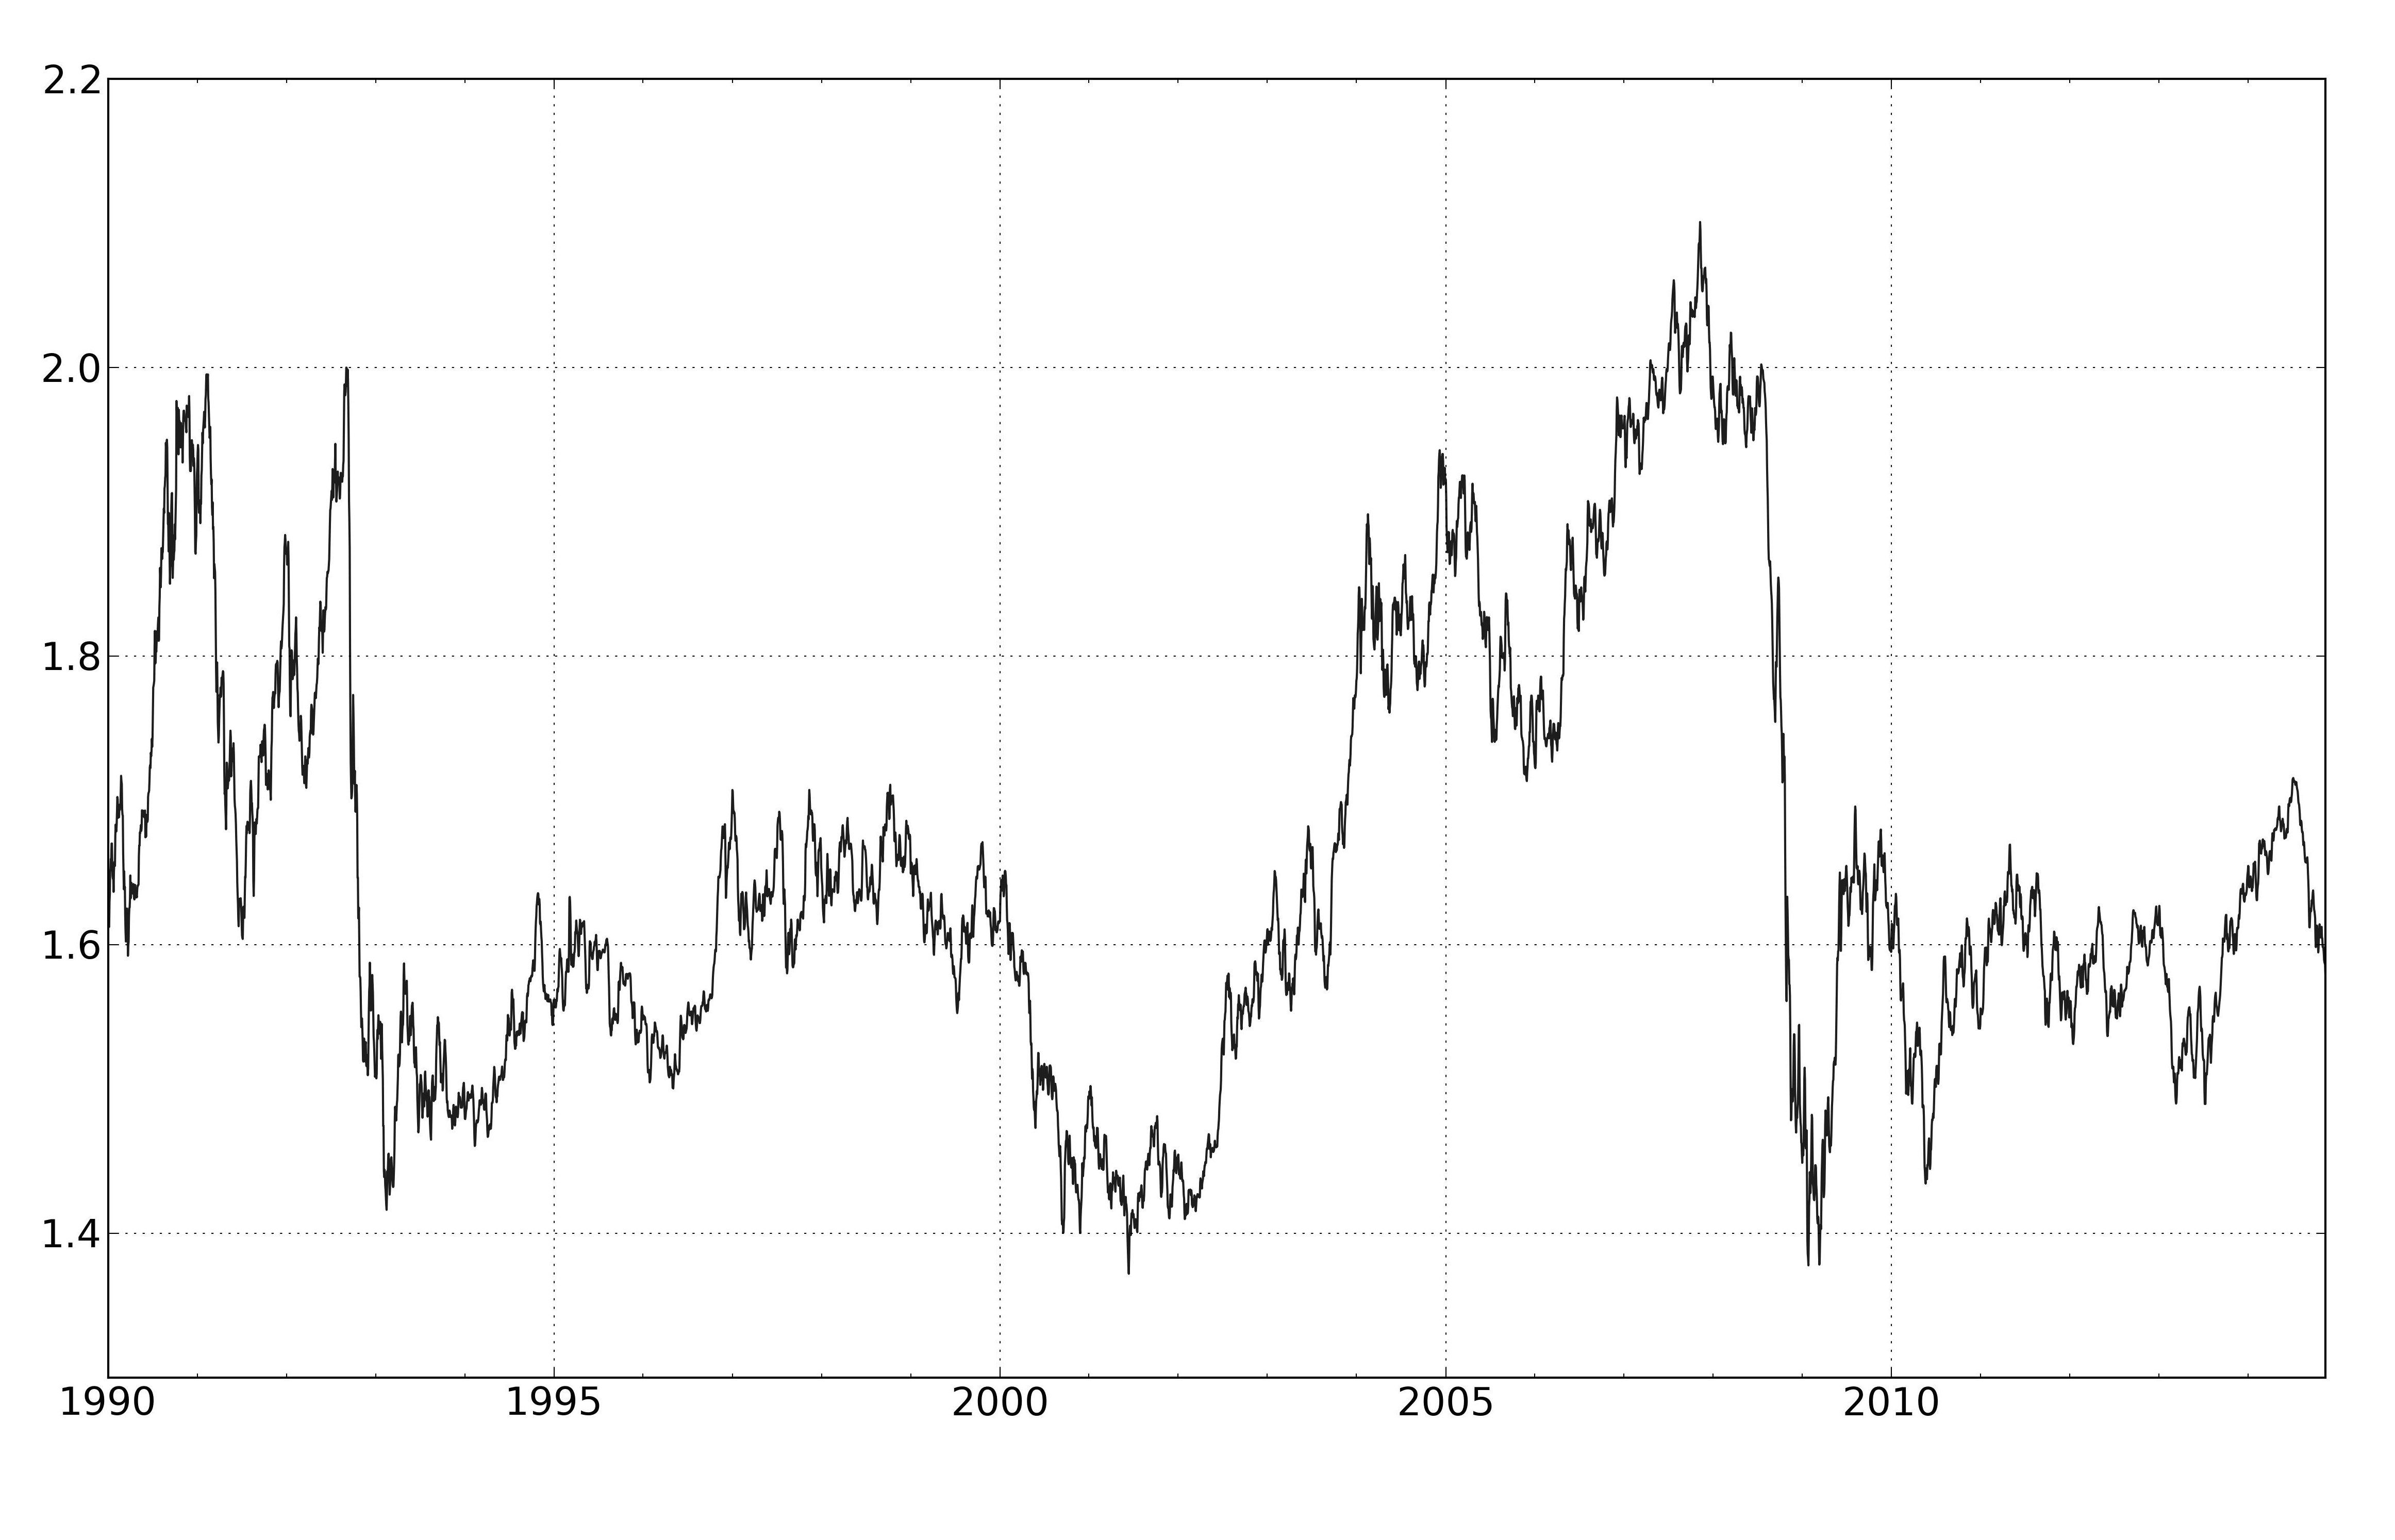
\includegraphics[width=\textwidth]{figures/raw/img-006.png} \caption{GBP vs USD exchange rate.} \end{figure}

During calibration you examine some \textbf{variations} on the basic trading rule. In the simple example you could test the original range of plus or minus 5\% against alternatives such as 3\%, 6\% or 10\%; or you can compare the current price against the average price over the last year, or week, or two years and so on. Usually you would choose the most profitable rule using a performance measure like the \textbf{Sharpe ratio}. Calibration can also be used --- as I will show later in the book --- to find rules which behave in a given way, such as trading at a given speed. You can then decide which variation, or variations, to keep.

Once you have chosen a portfolio of trading rules and variations you need to decide how to allocate your capital amongst them. Portfolio allocation decisions like this are the subject of the next chapter. For the moment it's worth noting that a poor variation can be rejected out of hand, or given a relatively small allocation in the overall system.

What if you want to use data first methods? Then you will need to be sufficiently expert to apply the principles in this chapter with your own preferred tools.\footnote{The main danger of the data first process is that you allow too many degrees of freedom. (I will not be defining this term since anyone using a data first approach ought to understand it already. If you don't you're in trouble!) Whereas the danger of ideas first is that you test too many ideas, or variations of ideas, until you find one (or 50!) that work. Either approach can result in over-fitted trading rules which look great in back-test but underperform once actually trading.} You should not use a data first method for which you don't have any deep understanding. I strongly suggest that you do not use a method blindly, just because it came packaged with some \textbf{back-testing} software.

Before we continue here's a final note of caution about ideas first testing. Any worthy trading systems designer will know their history, have read all the right textbooks and be aware of what other people trade. You could end up testing only ideas that you already know will work, which is a form of implicit \textbf{over-fitting}. As a result no matter how careful you are with the subsequent fitting process your back-tested \textbf{Sharpe ratios} will probably still be overstated --- beware overconfidence!

\subsection*{Cheating with a time machine}

Let's consider the first common mistake when fitting, which is pretending that you had access to a time machine.

When fitting there are always two distinct time periods. First there is the period used to fit the model, and secondly the time period used to test it. To illustrate this consider again the example of trying to fit a GBPUSD trading rule, and assume you're trying to find the best single variation. Suppose you've got ten years of daily price data available to fit on.\footnote{Throughout this book I'm going to assume that you are using daily data. This often means you can get longer histories of prices and it is appropriate for the kinds of trading rules I'll be discussing. Having data at a higher frequency is only necessary if you're testing very fast trading rules, such as those that expect to hold positions for less than a week.}

The easiest and probably most common method is to use the whole ten years as your fitting period, and find the single most profitable variation over that decade. You then go back and test how this single variation did over each of the same ten years. For each year that you are testing in, you use the same model, based on the entire ten years of data.

Figure 7 shows this for an example model running between 1990 and 2000. Each stage of the fitting occupies a row. So the first row shows that you would use all the data from the years 1990--2000 to fit the model which you test in 1990. In stage two you use the same fitted model to test performance in 1991, and so on.

The performance of this \textbf{back-test} will be amazing; too good to be true. Since no time machine was really available you didn't actually have the whole ten years of data in 1990 and you wouldn't necessarily have chosen the right variation. This is known as an \textbf{in sample} back-test because you are using the same data to fit and test performance. In sample testing should be avoided as it will produce extremely optimistic back-test results, and favour more complex rules that fit the data better but won't do as well in real trading.

There are better alternatives. A common one is to split the sample into two historical periods as in figure 8. You take all the data from the first half, 1990 to 1994, and fit the best variation over that period. Then you use that single variation to test your performance on the second \textbf{out of sample} period, which in this case is each year from 1995 to 2000.

The problem with this is that you waste half your data, and end up with only six years of performance to look at.\footnote{You can also fit on the first half of the data and test on the second half as before, and subsequently fit on the second half and test on the first. This keeps more data but isn't entirely honest as it still requires a time machine, albeit one you use only once. Yet another variation is to use the entire dataset to fit except for the year you are testing. This also strikes me as relatively dishonest.} You also don't account for any potential changes in market structure in the second half of the data.

\begin{figure}[htbp] \centering 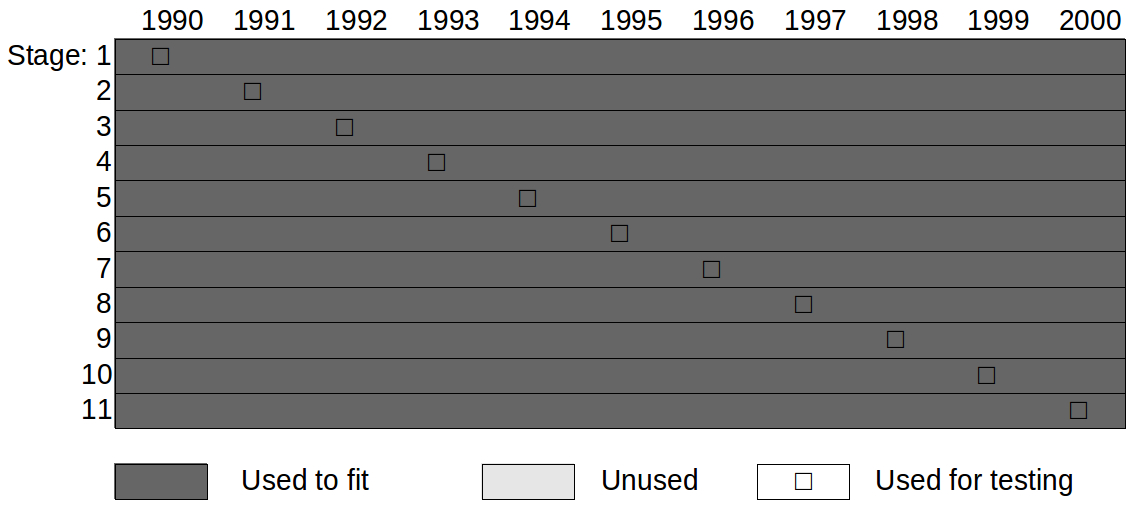
\includegraphics[width=\textwidth]{figures/raw/img-007.png} \caption{In sample back-testing: efficient but dishonest.} \end{figure}

In sample testing. You use all the data to fit and then test performance from the start. In each stage (row) you test data for a different year, but use data from all years to fit.

\begin{figure}[htbp] \centering 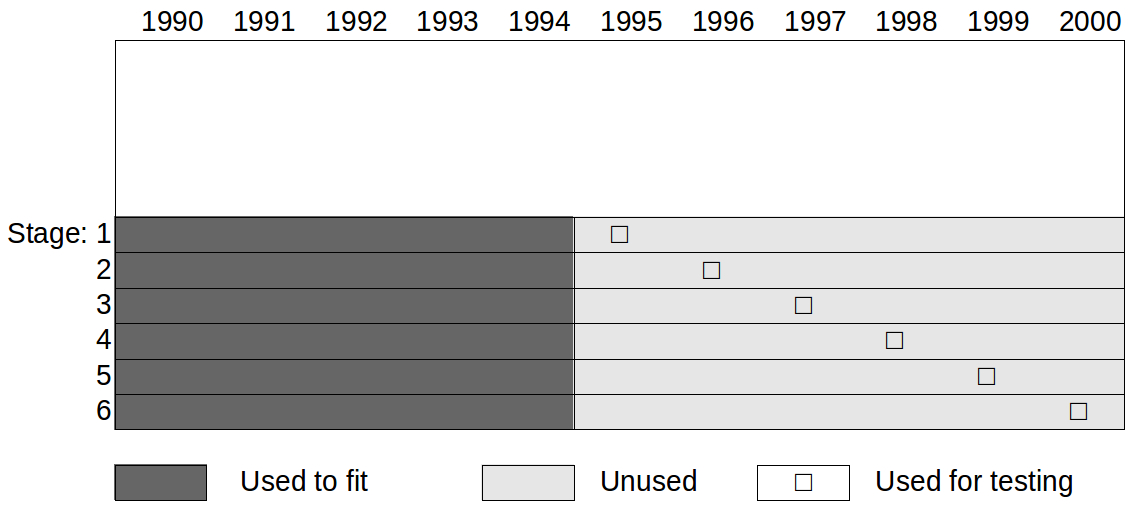
\includegraphics[width=\textwidth]{figures/raw/img-008.png} \caption{Half out of sample testing: honest, but wasteful.} \end{figure}

You fit your trading rules on the first half, and then test performance on the second half. In each stage (row) you test a different year, but always using the first half of the data to fit. No testing is done in the first half of the data. The second half of the data isn't used for fitting.

My preferred solution is to use an \textbf{expanding} window, as in figure 9.\footnote{This is sometimes called anchored fitting.} Suppose you think you need at least a year to fit your system. In the next stage you fit on the first year of data for 1990, and then test the resulting variation in the second year, 1991. Then in stage three of figure 9 you test in 1992 using the variation fitted with data from the years 1990 and 1991. To test 1993 you use the best variation fitted using 1990, 1991 and 1992.

This continues until 2000 when you're using the previous ten years of data to select the best variation. Because you only fit using the past you're not cheating. You also use as much of the past as you ``legally'' can, so nothing is wasted.

The only problem with this method is that if the world changes you'll still be using potentially irrelevant past data. To avoid this you could fit on the last five or ten years of data, once you have enough history to do so, and discard earlier years. This is a \textbf{rolling window}.\footnote{Another widely used term for this is walk forward fitting.} As figure 10 shows a five-year rolling window is identical to the expanding window until 1996. At this point you would discard 1990, and use only the years 1991 to 1995 to fit the best variation.

The length of the window needs to be short enough to pick up changes in market structure, but long enough to give statistically significant results. As you'll see later you often require multiple decades of data to fit models, which makes the use of rolling windows problematic.

\begin{figure}[htbp] \centering 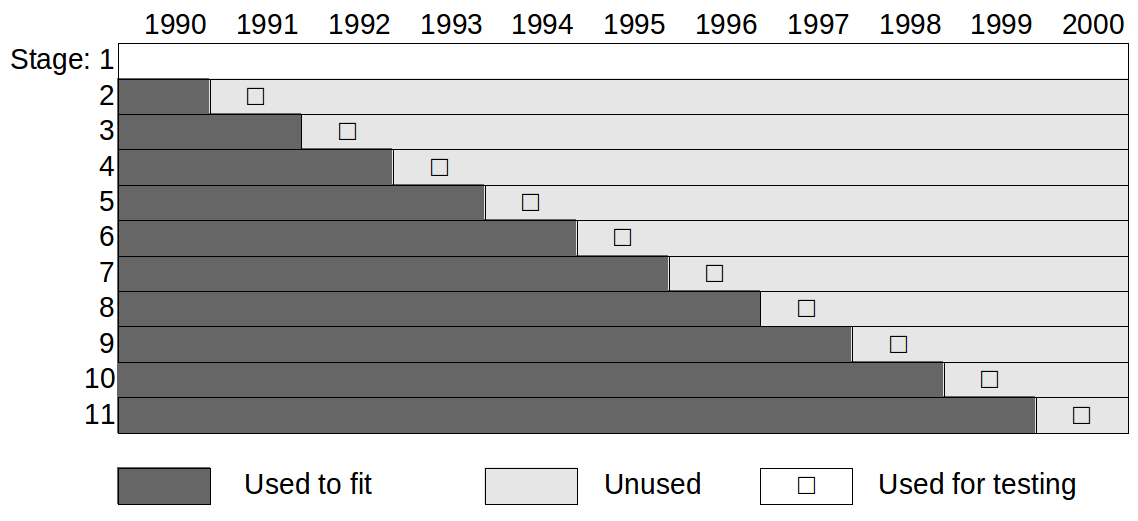
\includegraphics[width=\textwidth]{figures/raw/img-009.png} \caption{Expanding out of sample is both efficient and honest.} \end{figure}

Every year you fit the data only on the past. Each row shows the fitting and testing done for a particular year.

\begin{figure}[htbp] \centering 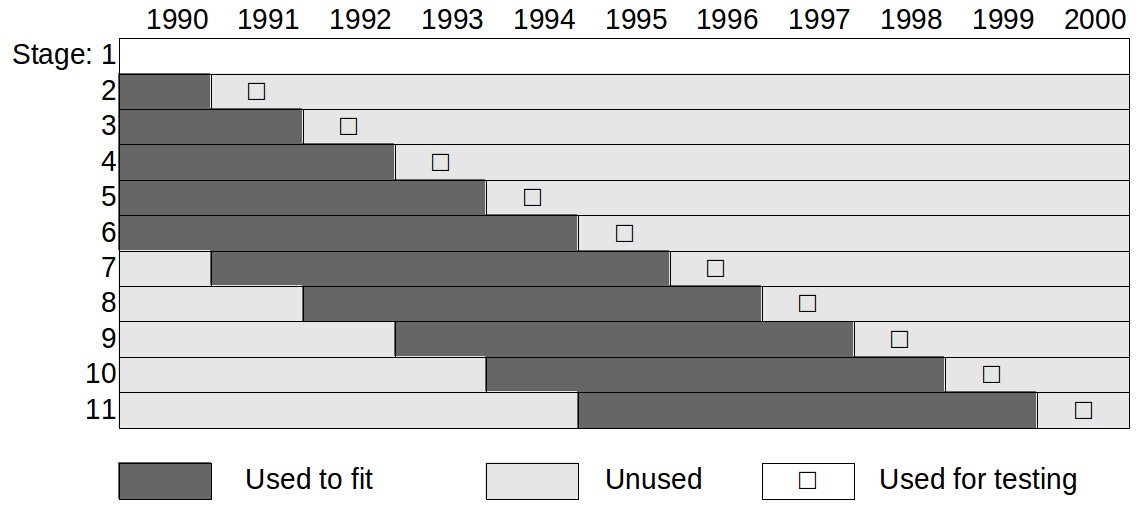
\includegraphics[width=\textwidth]{figures/raw/img-010.png} \caption{Rolling out of sample adapts to changing conditions, but make sure you have enough data for statistical significance.} \end{figure}

Every year you use the past data to fit; up to five years' worth. Each row shows the fitting and testing done for a particular year.

\subsection*{When fitting goes bad}

Now let's examine a concrete example of poor fitting practice. I'm going to select the best \textbf{variation} of the early loss taker \textbf{trading rule} I introduced in chapter one to run over the CME gold futures contract, out of a possible menu of 90 variations.\footnote{For those who are interested this is based on the ``A and B'' system defined in appendix B. Values for B (the stop loss value) will be the integers from 1 to 10; to capture different trend lengths. Because I only want to look at trend following rules (early loss takers) I iterate only over values of A (the profit target) that are equal to or larger than B: $A = 1 \times B$,$1.5 \times B$, $2 \times B$, ... $5 \times B$. This gives 90 possible variations in all.} This might seem excessive, but it's fewer variations than Joe was testing in my earlier anecdote. Bear in mind that if I had a five parameter trading rule, and I allowed each parameter to take one of ten discrete values, then I'd be testing 10,000 variations!

Once I have at least one year of data I find the highest performing variation based on the \textbf{Sharpe ratio (SR)} from the previous 12 months. I then test the performance for the following year, again using the last 12 months of data. This process is then repeated annually. You should recognise this as a one year \textbf{rolling window back-test}.

Which of the following alternatives do you think will give me the best performance?

\begin{enumerate}
\item Picking the best variation: Each year I use the best performing variation from the previous year.
\item Picking a random variation: Ignoring my fitting, each year I choose one variation at random. Because the randomness of each choice will influence the results I run this experiment a number of times, and take the average performance.
\item Keeping all the variations: Again ignoring my fitting, I keep all 90 variations, and use an equally weighted average of their forecasts. \end{enumerate}

If you're a big fan of fitting the results are disappointing. Choosing the best rule each year from the previous year gives me a rather poor SR of 0.07. If I go for the second option and just choose a random rule annually each January 1st, then on average I get a Sharpe of 0.2. The best option is to forget about selecting trading rule variations entirely and run an equal blend of them all. This gives an SR of 0.33, which is pretty good for one kind of trading rule run on a single \textbf{instrument}. These results could be a fluke but I get similar results on many different instruments and trading rules.

Why does fitting do so badly?

Firstly choosing just one variation to run at a time smacks of overconfidence. As you'll see shortly we rarely have enough evidence that one rule is definitely better than another. Secondly one year of data is wholly insufficient to decide which trading rule is best. I make this problem worse by fitting on the history of a single instrument, gold futures. Finally, like Joe, I am testing far too many variations.

\subsection*{The hazards of rule selection}

\subsubsection*{The multiple testing problem --- even some random rules will look good}

Why is it so dangerous to test large numbers of \textbf{trading rules} and \textbf{variations}? Apart from the effort involved it's very likely that you will end up picking a poor rule just by chance.

To see why here is an experiment. Let's suppose I am trying to achieve alchemy and find profitable rules where there are none to be had. I have a pool of a certain number of possible trading rules, all of which have true expected average returns of zero, although in a real scenario I wouldn't know this beforehand! The rules are entirely arbitrary and their returns are generated from random data.\footnote{Many of the examples in this chapter will use imaginary daily returns of various arbitrary trading rule variations. These fake returns are randomly generated with the kind of characteristics I want: expected mean, standard deviation (from which we get the Sharpe ratio), and where relevant correlation with other variations. I then run these tests many times and report the average result, so the answer is not influenced by how each series of random numbers come out.}

For each test I get one year of return data for each rule in my pool, as in the gold futures example above, and select all the rules whose \textbf{Sharpe ratio} (SR) in that year is higher than a given minimum level. If no rule has an SR above the threshold then I won't choose any. All the rules that pass the test will be kept (even if there are 50!).

Because the underlying data is random I need to generate new data multiple times and then repeat the test to get meaningful results. I then measure the average number of rules accepted given a specific minimum level and the size of the pool available. As table 3 shows, even if I'm strict and set an extremely high minimum SR of 2.0 I'll still pick up a couple of bad rules if I test enough of them.

\begin{table}[htbp] \centering \small \caption{If you test enough rules, some bad ones will always slip through} \begin{tabular}{@{} lccc@{}}
\toprule
Number of rules tested in pool & 0.5 & 1.0 & 2.0 \\
\midrule
1 & $<1$ & $<1$ & $<1$ \\
5 & 1.4 & $<1$ & $<1$ \\
10 & 3 & 1.5 & $<1$ \\
50 & 16 & 8 & 1.2 \\
100 & 30 & 16 & 2.3 \\
\bottomrule
\end{tabular}
\end{table}

The table shows the average number of rules accepted from pools of arbitrary unprofitable rules, given different pool sizes (rows), which were tested to see if their Sharpe ratio exceeded a minimum cutoff (columns).

Practically then what SR cutoff should I use? As none of the imaginary rules are truly profitable ideally I wouldn't accept any. But in real fitting situations we can't set the bar too high or even good rules will be discarded; after all a realistic SR for a real trading rule, tested on one \textbf{instrument}, is only likely to be around 0.30. Let's suppose I would be happy with a 5\% chance of picking out at least one rule that was truly unprofitable. Also in the real world I'd usually have more than one year of data, so let's see what effect additional history has on my findings.

Table 4 has all the results. As you might have suspected the length of the return series is very important here. More history means less chance of a zero SR rule getting a lucky streak, so I can set the cutoff lower. However, even with 30 years of data I can't risk testing more than a handful of rules, and even then the cutoff is far too high when many perfectly good variations will only have true Sharpe ratios of 0.3.

\begin{table}[htbp] \centering \small \caption{With more history you can set a lower Sharpe ratio threshold to avoid picking a bad rule from a larger pool} \begin{tabular}{@{} lcccc@{}}
\toprule
Number of rules tested & 1 & 5 & 10 & 30 \\
\midrule
1 & 1.5 & 0.7 & 0.5 & 0.4 \\
5 & 2.3 & 1.1 & 0.8 & 0.5 \\
10 & 2.8 & 1.2 & 0.8 & 0.6 \\
50 & 3.4 & 1.5 & 1.0 & 0.6 \\
100 & 3.4 & 1.5 & 1.1 & 0.7 \\
\bottomrule
\end{tabular}
\end{table}

The table shows the Sharpe ratio cutoff needed when testing a given size pool (rows) of trading rules, with a certain amount of years of historical data (columns) to ensure you only have a 5\% chance of picking out one or more truly bad rules.

\subsubsection*{How much history do you need to decide if a rule is good?}

You've now seen that a common mistake is to use insufficient historical data to select or calibrate a rule. How much data do you need? How long do you need to decide if a rule has a positive \textbf{Sharpe ratio} (SR) and is worth keeping?

To answer this I generated more random trading rule daily returns, this time assuming an underlying positive Sharpe ratio, which again I wouldn't know in advance. As more trading history is generated I can estimate the SR each year and the average so far. At the same time I look at the distribution of those annual Sharpe ratios.\footnote{For a more technical discussion of this issue, see Andrew Lo's paper ``The Statistics of Sharpe ratios'' in \textit{Financial Analysts Journal} 58:4, July/August 2002.} This allows me to get a feel for how statistically significant my measured average SR is; was I just lucky or is this really a good system?

A classic test for statistical significance is the T-Test. In this example it determines whether an estimated Sharpe ratio is likely to be positive given the estimate of its mean and \textbf{standard deviation}. The further away the mean is from zero, as measured in units of \textbf{sigma}, the more likely the unknown SR is actually positive.

This test is commonly used with a threshold of two \textbf{sigma}. If an estimated average SR is more than two standard deviations above zero there would only be a 2.5\% chance of this happening if the true SR was actually negative.

Figure 11 shows the evolution of the average measured SR for an arbitrary trading rule, and around it the upper and lower ``confidence intervals''. Each confidence interval is two \textbf{sigma} away from the average, so when the lower interval pushes above zero I know there is only a 2.5\% chance the trading system is really a loss making rule in disguise.

\begin{figure}[htbp] \centering 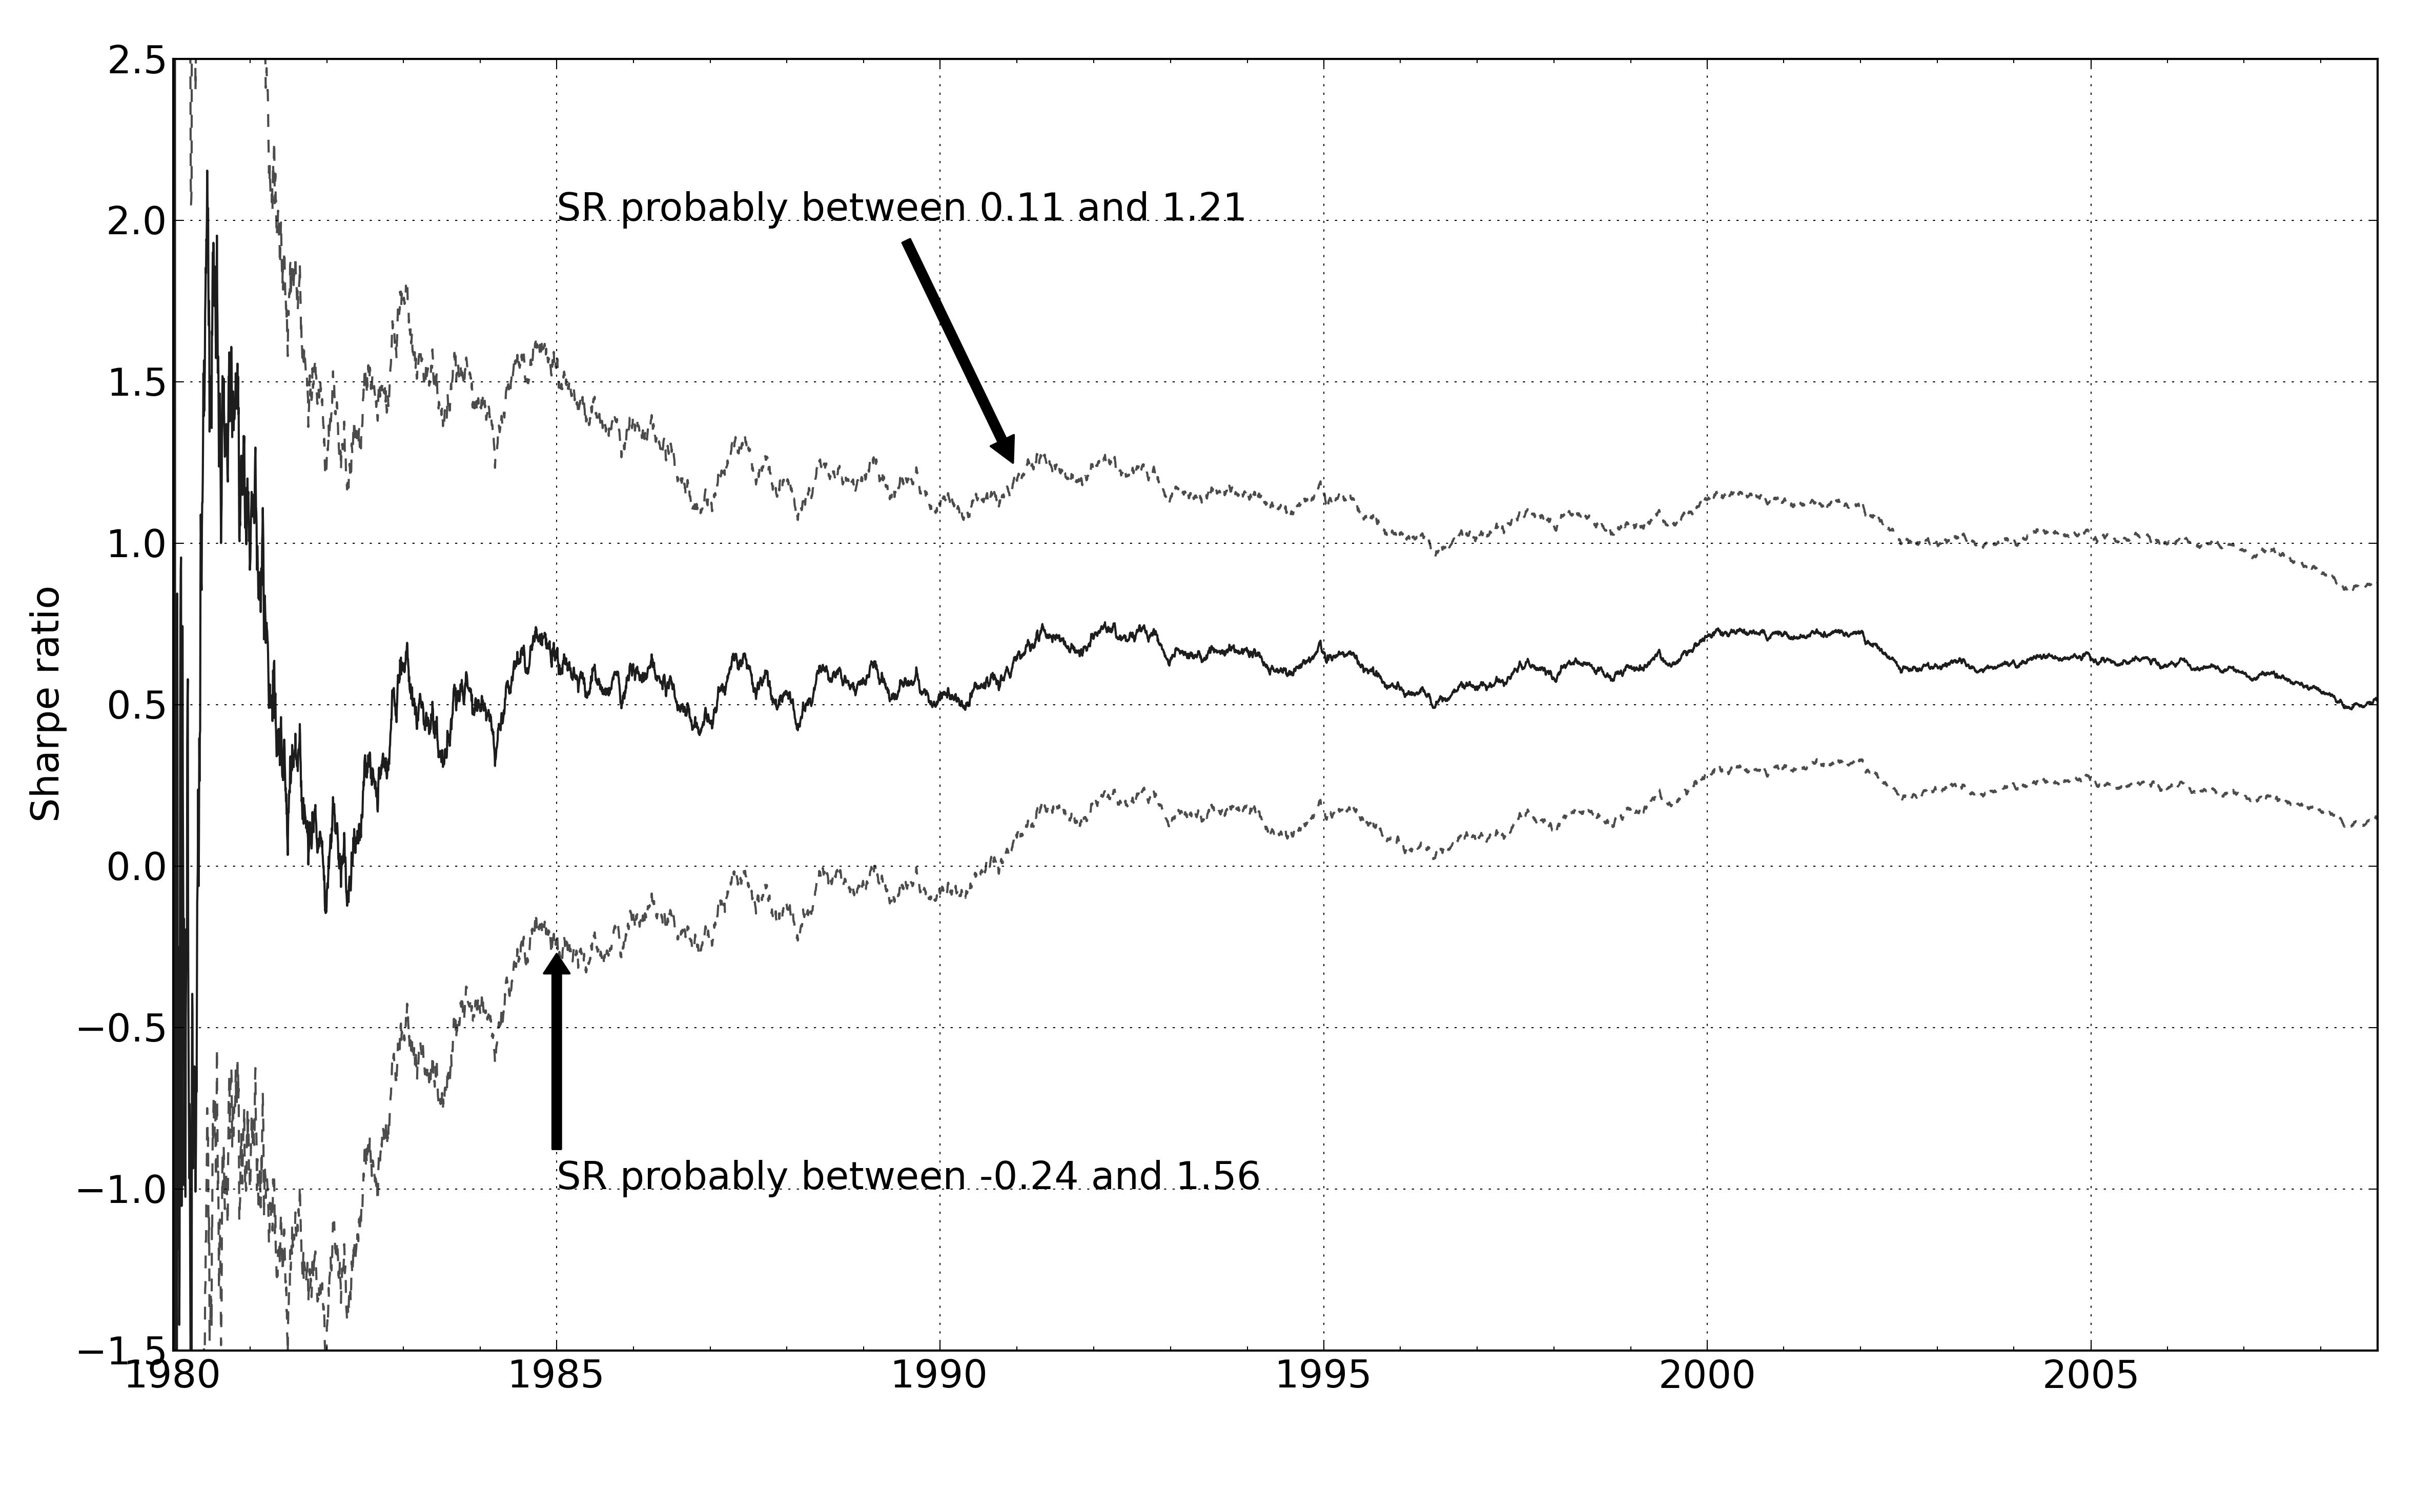
\includegraphics[width=\textwidth]{figures/raw/img-011.png} \caption{With a true Sharpe ratio (SR) of 0.5, it takes more than ten years to pass the T-Test and conclude the SR is probably positive.} \end{figure}

In the figure you can see the average SR converging quickly on the true value of 0.5 SR. But it takes over ten years before the lower confidence interval goes above zero and the T-Test is finally passed. Only then can we be reasonably certain this is not a loss making system.

If I repeat this for a rule with a true SR of 1.0 I get figure 12. The time to pass the test here is just a few years. On average it will always take less time for higher SR strategies to prove their profitability.

\begin{figure}[htbp] \centering 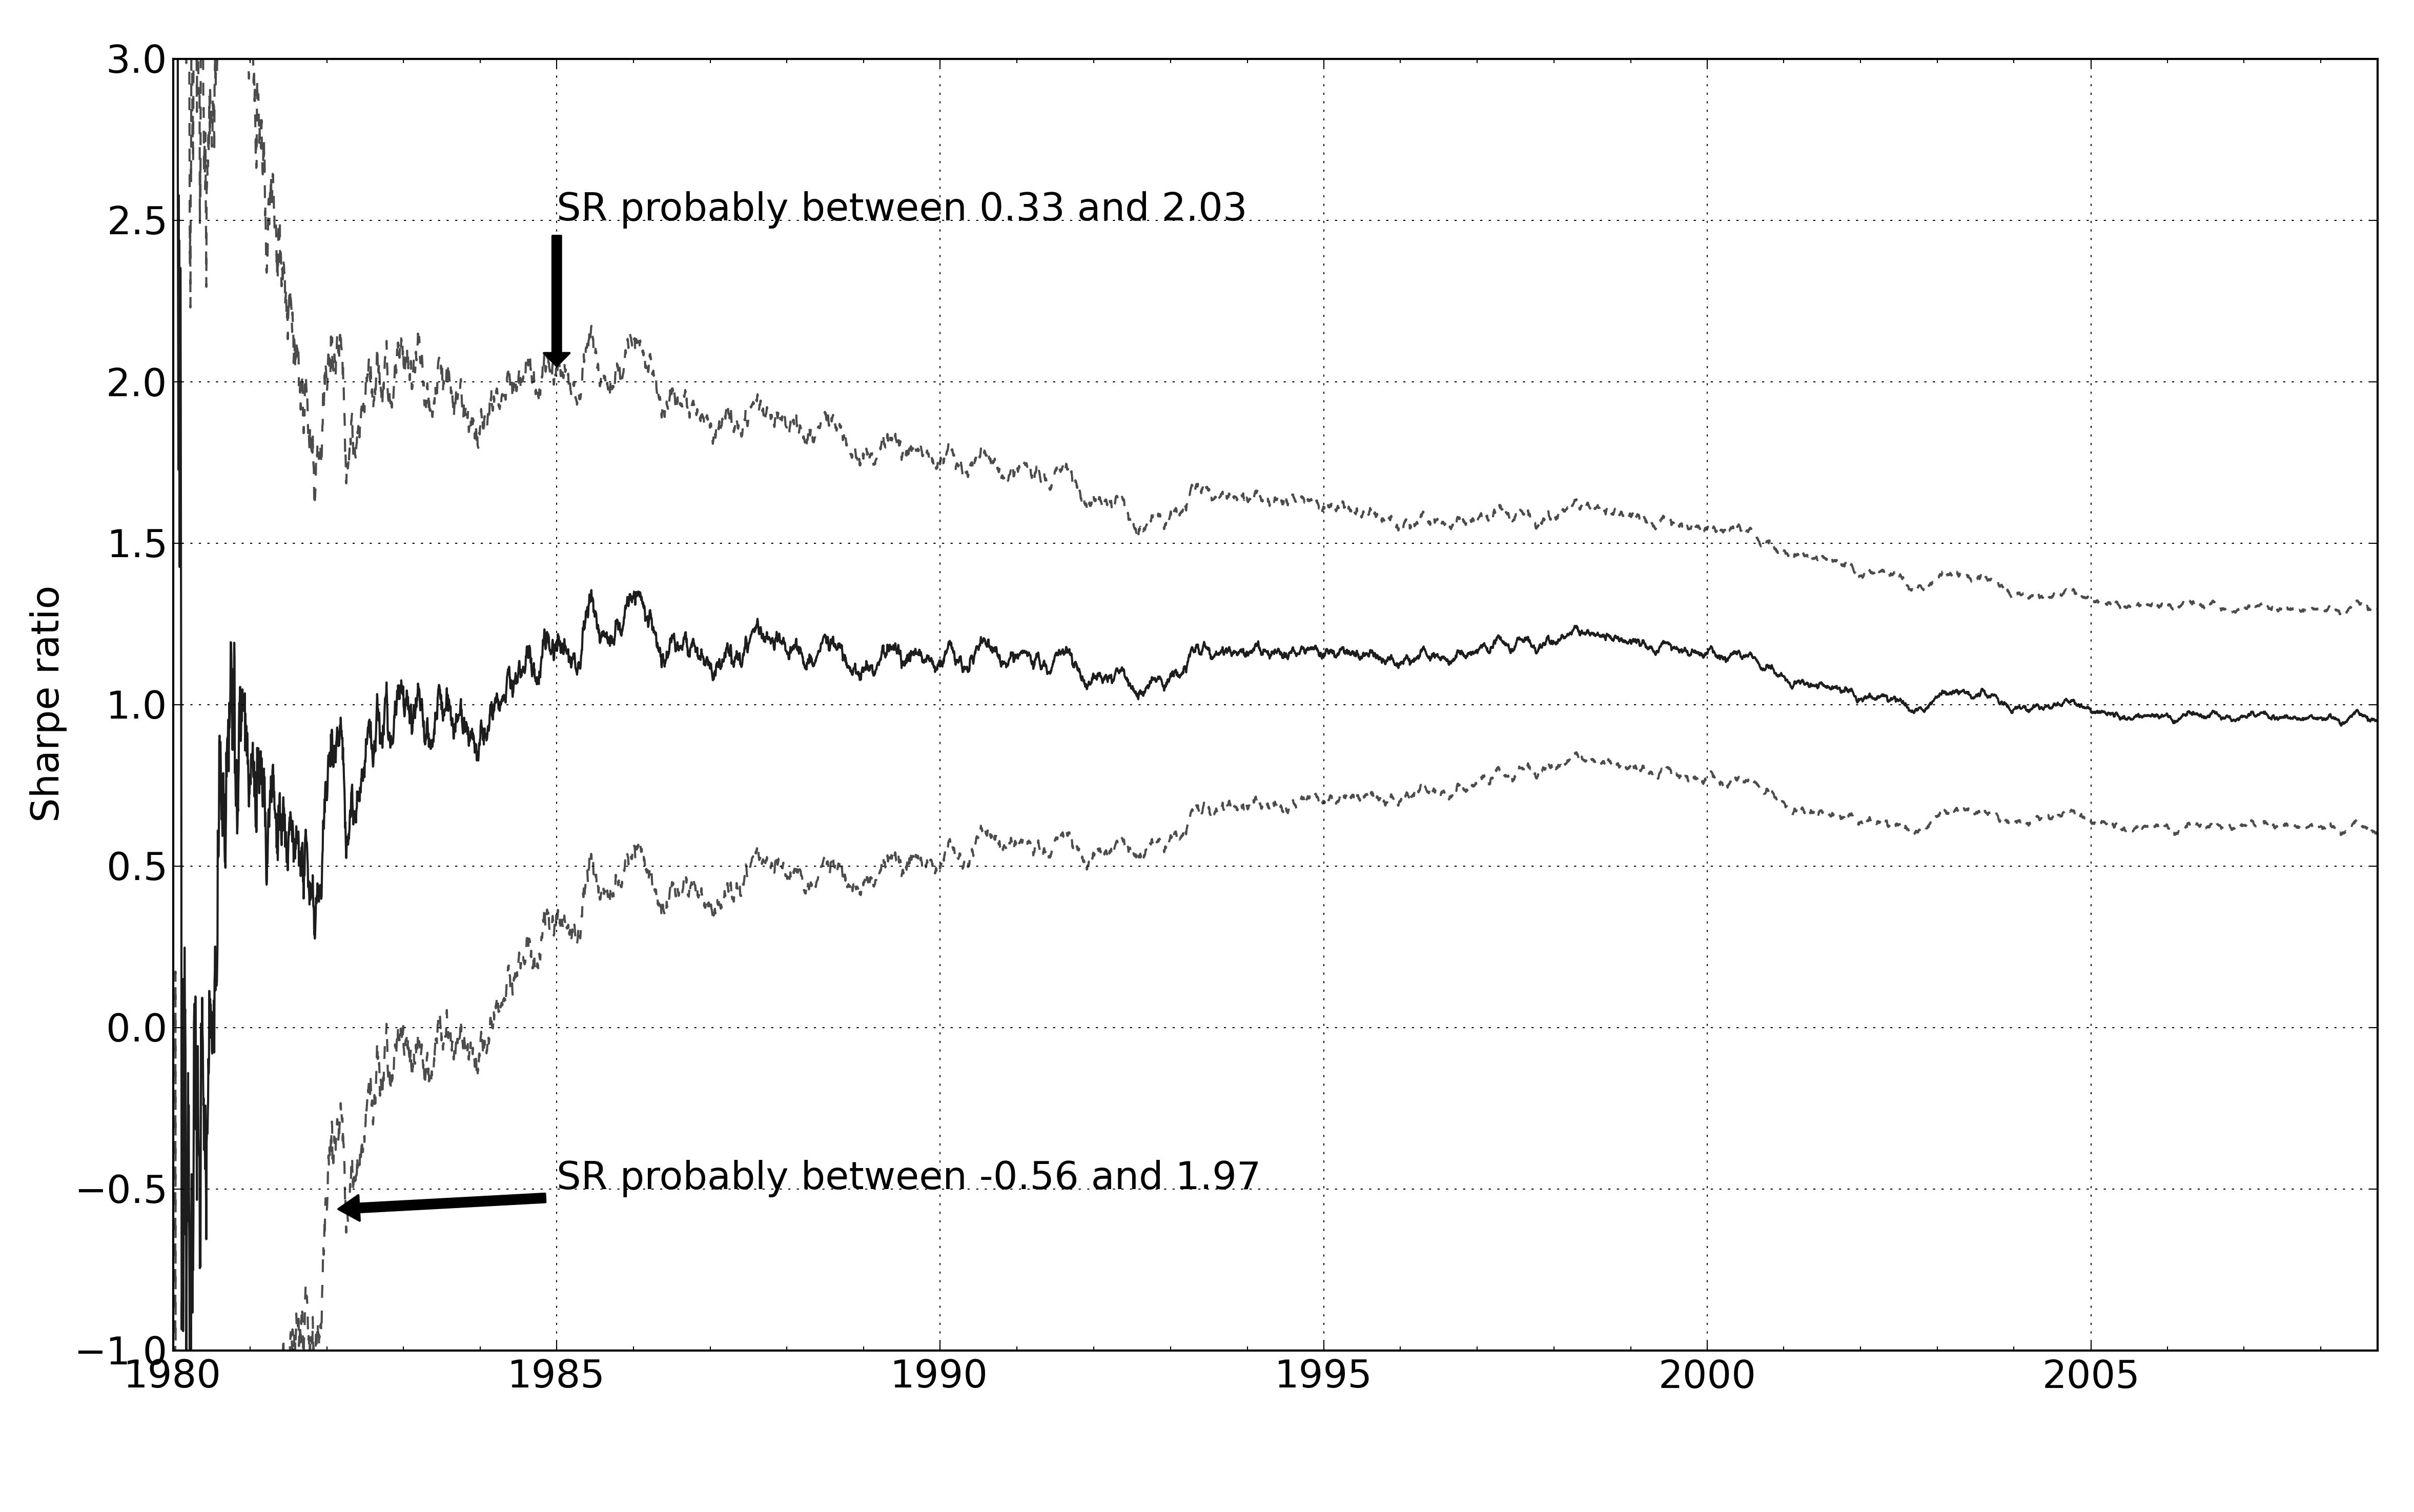
\includegraphics[width=\textwidth]{figures/raw/img-012.png} \caption{With a true Sharpe ratio of 1.0 we pass the T-Test in a few years.} \end{figure}

Let's find the average time to pass the test for a given true Sharpe ratio. After running the necessary experiments I get table 5. Except for very good rules you need at least ten years, and usually more, to be sure a strategy makes money.\footnote{These results also depend on the \textbf{skew} of returns. For example, with a true SR of 1.0 I needed about three years' more data for a typical negative skew volatility selling strategy to pass the T-Test, compared to a positive skew \textbf{trend following} strategy.} The average trading rule for one \textbf{instrument} has a realistic SR of around 0.3; so you'd need nearly 40 years of history!

\begin{table}[htbp] \centering \small \caption{It takes decades of data to see if most strategies are likely to be profitable} \begin{tabular}{@{} lcccccccc@{}}
\toprule
True Sharpe ratio & 0.2 & 0.3 & 0.4 & 0.5 & 0.7 & 1.0 & 1.5 & 2.0 \\
Average years to pass profit T-Test & 45 & 37 & 33 & 20 & 10 & 6 & 3 & 1.4 \\
\bottomrule
\end{tabular}
\end{table}

The table shows average time in years to pass the T-Test for profitability given the true Sharpe ratio of the trading rule.

\subsubsection*{How much history do you need to decide if one rule is better than another?}

Now what if you have some alternative rules and want to find the best. Let's suppose I again have two random rules, one with a true \textbf{Sharpe ratio} (SR) of 0.30, and the other an SR of 0.80. Initially I'm going to assume these are quite different rules with no \textbf{correlation} between their returns. This time to perform the T-Test I need to estimate the difference in the two Sharpe ratios, and measure the average and standard deviation of that difference.

\begin{figure}[htbp] \centering 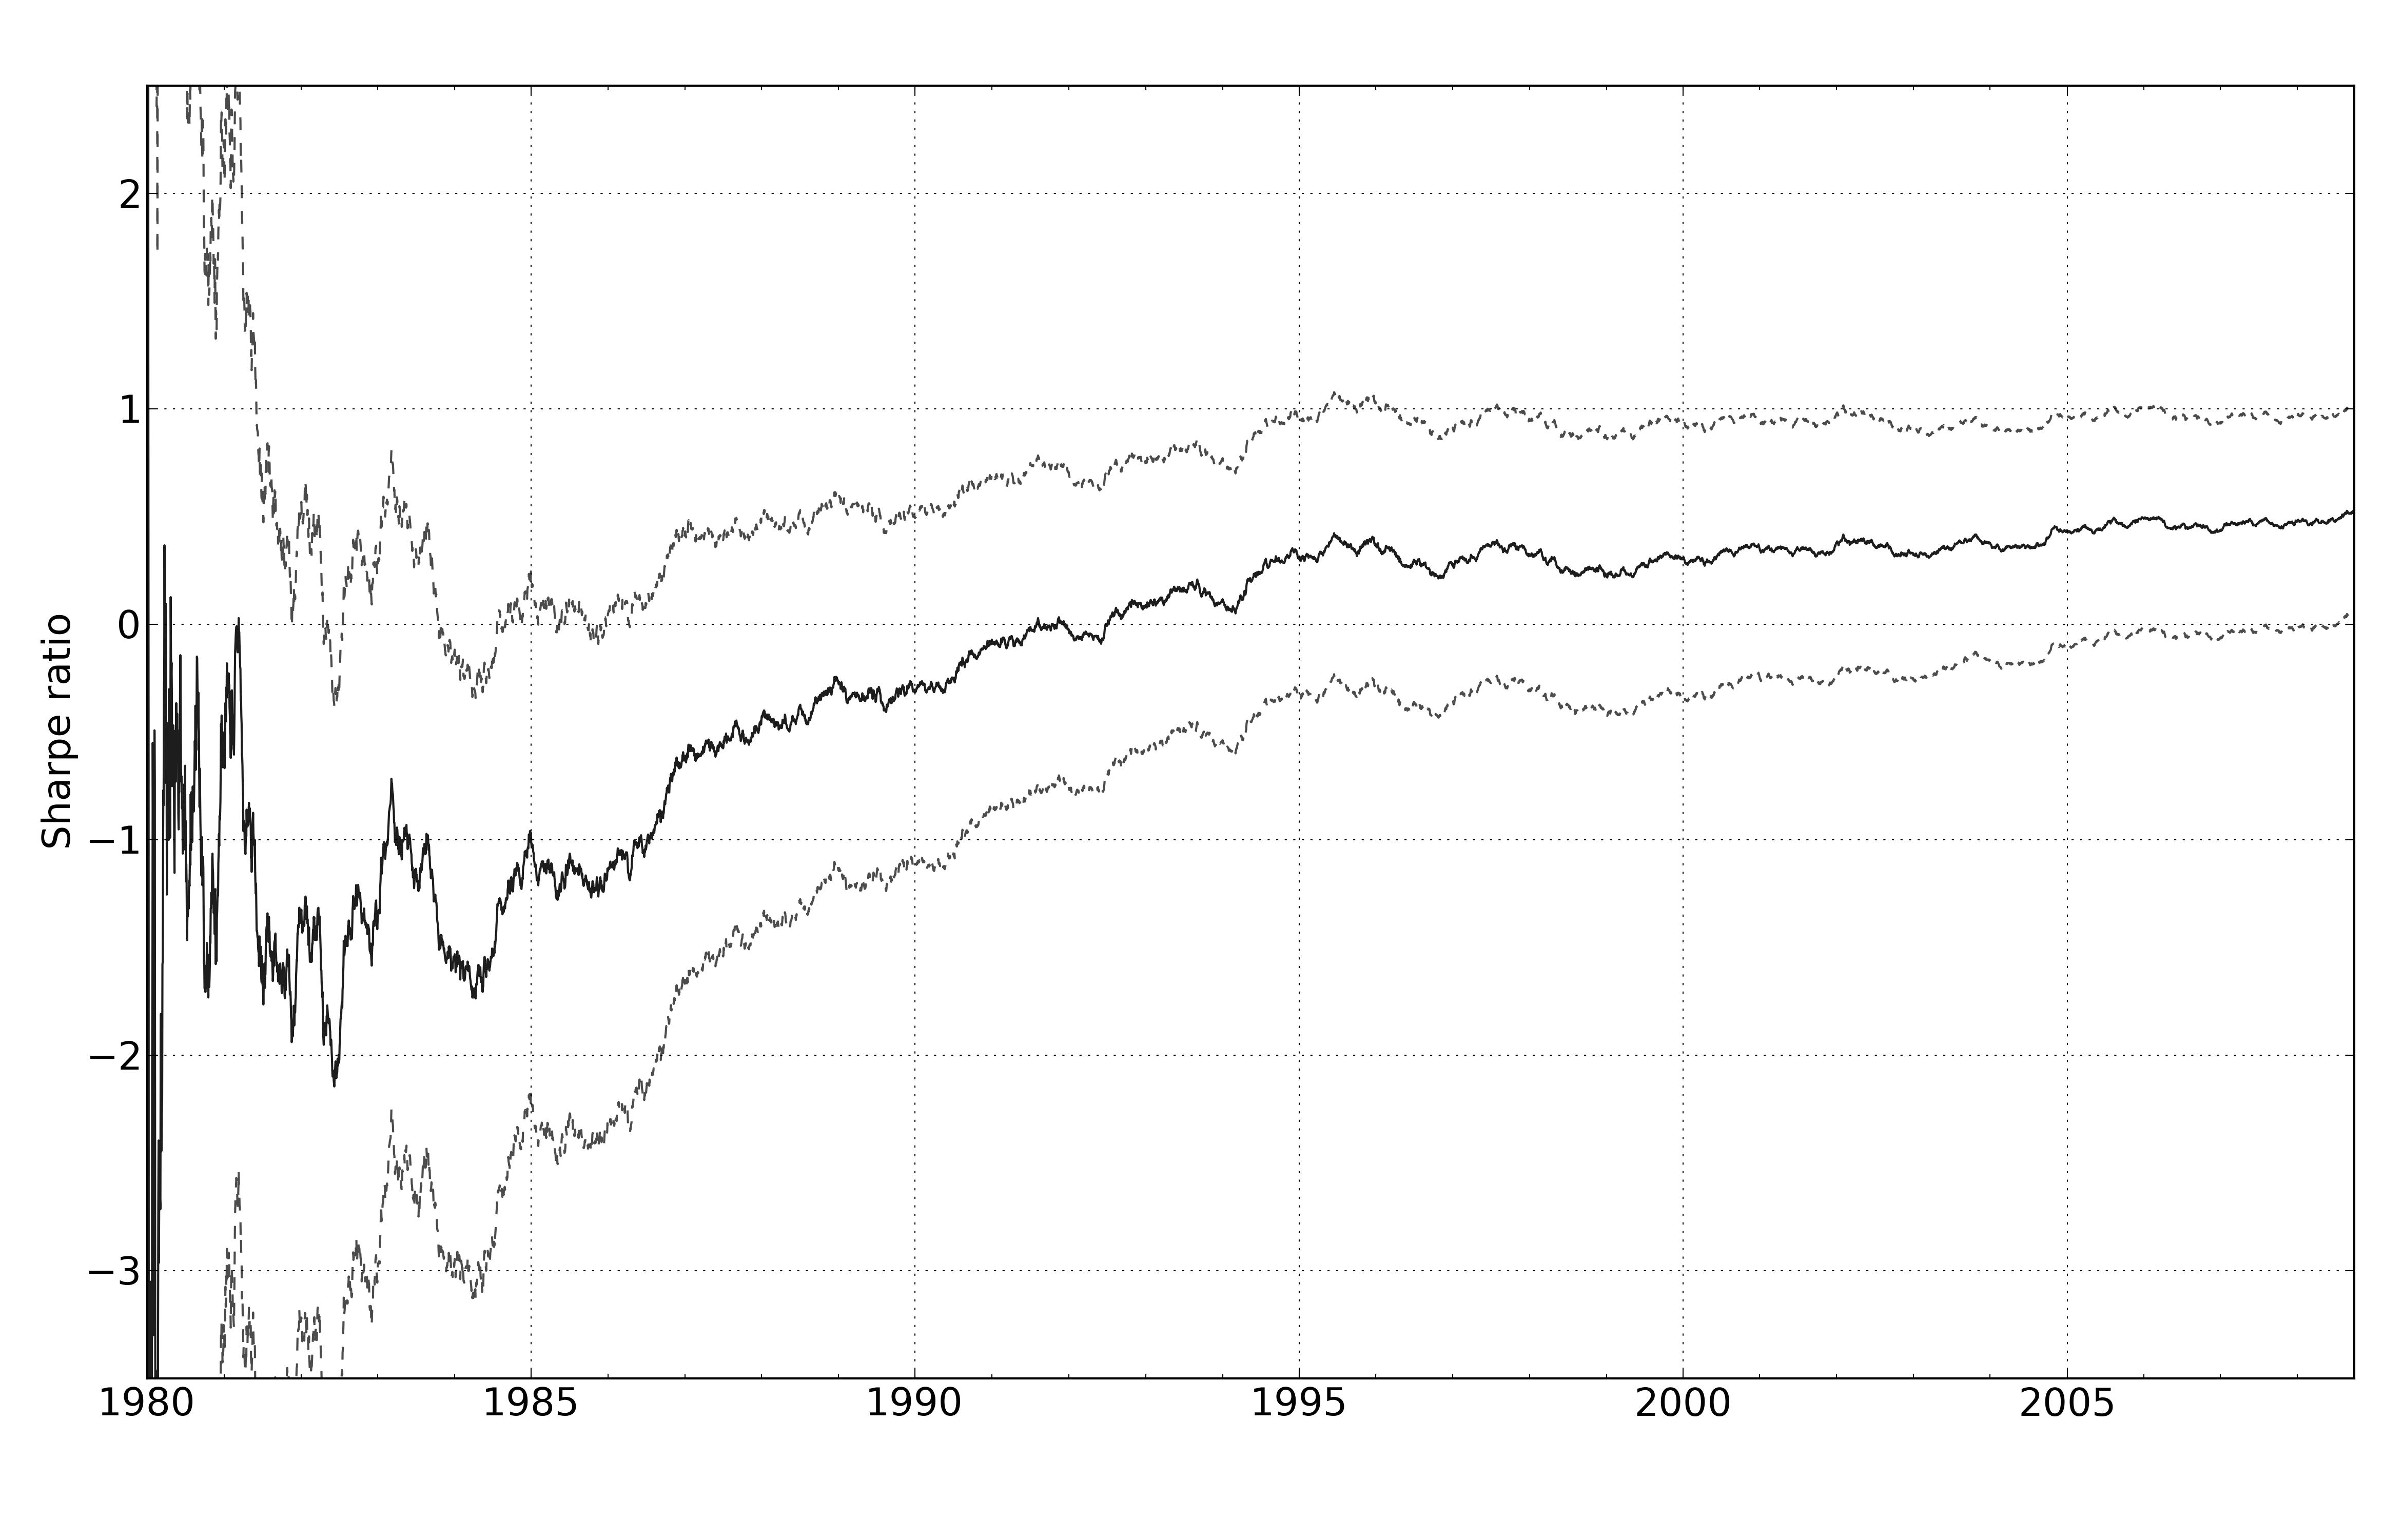
\includegraphics[width=\textwidth]{figures/raw/img-013.png} \caption{It takes three decades to discover that this SR 0.8 strategy is probably better than an uncorrelated strategy with SR 0.3.} \end{figure}

In figure 13 is the average difference in SR and the relevant confidence intervals for this difference. Once the lower confidence interval goes above zero then we can be reasonably certain that one rule is better, as again there is only a 2.5\% probability of this happening by chance. You can see from figure 13 that the time to certainty is around 30 years!

Table 6 shows the average time taken to pass the T-Test when comparing an SR 0.30 rule with one that truly has a higher SR. These results vary depending on the difference in SR and the correlation of the rules. More closely related rules will be easier and quicker to distinguish for a given SR difference.\footnote{More subtly the overall level of the Sharpes involved will also influence the results, as Andrew Lo's paper discusses. The skew of the rules is also important, even when comparing rules with similar skew.} In practice distinguishing rules requires considerable historical data except for the rare cases of variations which are both highly correlated, and also perform very differently.

\begin{table}[htbp] \centering \small \caption{Can you distinguish trading rules given a few years of data? Only if they are highly correlated and one heavily outperforms the other} \begin{tabular}{@{} lccccc@{}}
\toprule
Sharpe ratio advantage & -1.0 & 0.0 & 0.5 & 0.8 & 0.95 \\
\midrule
0.1 & 47 & 47 & 46 & 44 & 37 \\
0.25 & 46 & 45 & 40 & 32 & 10 \\
0.5 & 41 & 37 & 25 & 10 & 3 \\
1.0 & 23 & 11 & 8 & 2.5 & 0.5 \\
\bottomrule
\end{tabular}
\end{table}

The table shows the number of years needed for us to be reasonably certain that one rule is better than another, given the SR advantage of the better rule (rows) and the correlation between the trading returns of the two rules (columns).

\subsubsection*{Should you fit one trading rule for all instruments?}

In 2010 the large systematic hedge fund in which I worked was reorganised into \textbf{asset classes}. My team managed the fixed income portfolio, another ran equities and so on. Initially the trading strategies we ran were fairly similar. However over time, as we did more market specific research, we all became convinced that we needed to customise our systems differently.

In many cases we went further and also began to fit different parts of our portfolios separately. We might for example have fitted emerging and developed market bond futures with different trading rule variations.\footnote{In reality we didn't do this. Or did we? Unfortunately I can't give real examples without breaking the terms of my non-disclosure agreement.} Fitting separately is common, and many system traders take this to the extreme and fit every \textbf{instrument} separately. Almost all \textbf{back-testing} packages, such as the one Joe was using, default to fitting trading rules on a single instrument at a time. So you would have one \textbf{variation} of a rule for the British pound/dollar, another for euro/dollar and so on.

This is a classic example of the narrative fallacy, a \textbf{cognitive bias} we have seen before. To our human minds it makes sense to have different stories, and so different trading rules, for different instruments.

But is this the right thing to do? It depends on whether the behaviour of each variation over the various instruments is significantly different. If it isn't then you're likely to be \textbf{over-fitting} by individually tailoring each rule for every instrument. In practice there isn't usually a statistical difference between different instruments, particularly if they are closely related such as a group of equity index futures.\footnote{There are some exceptions, notably when there are different trading costs for the instruments concerned, which I'll cover in chapter twelve, ``Speed and Size''.}

In fact pooling your data and fitting multiple instruments together is an excellent way of getting more data history, which gives you a better shot at being able to distinguish profitable and loss making trading rules.

As an example I have two trading rules in my own portfolio which for a typical single instrument have \textbf{Sharpe ratios (SR)} averaging 0.05 and 0.30 respectively. Despite being perfectly uncorrelated, table 6 shows I'd need 45 years to distinguish them; almost impossible when even the earliest financial futures only began trading in 1972. However the same rules run on a portfolio of instruments have SR of 0.13 and 1.13.\footnote{Technical note: These are the returns you'd get if you traded an equally weighted portfolio of instruments using the same trading rule. The improvement in \textbf{Sharpe ratio (SR)} comes from the diversification effect across instruments. The alternative method is to stitch consecutive series of instrument returns together. This gives a very long history of returns, but the SR of the stitched series will be almost the same as the average across individual instruments (it is not identical to the average because of the effect of varying lengths of price series for different instruments).} The table shows I'd need just 11 years of data to distinguish these two Sharpe ratios from each other.

To make pooling easier you should design trading rules that are generic and can work with any instrument. I'll give some examples of generic rules in chapter seven, ``Forecasts''.

\section*{Some rules for effective fitting} \phantomsection \addcontentsline{toc}{section}{Some rules for effective fitting}

If you haven't been warned off fitting, and insist on using data to select and calibrate trading rules, then following this advice should keep you out of serious trouble. Those who are now rightly terrified of fitting can skip ahead to the next section, where I show you how I avoid fitting almost completely.

\subsection*{Keep it simple}

I am not a fan of complex fitting methods and I prefer not to use them. But if you do consider yourself an expert in a dark statistical art then naturally you would want to practise it. Just be aware; the more complex the method the harder it will be to realise when you are \textbf{over-fitting}.

\subsection*{Fewer alternatives}

As table 4 shows reducing the pool of \textbf{trading rules} and \textbf{variations} considered is crucial unless you have many years of data.\footnote{If you are using a more complex fitting technique then you need to keep your degrees of freedom appropriately small.}

\subsection*{Ban time machines}

You should always use \textbf{rolling} or \textbf{expanding out of sample} fitting. If using a \textbf{rolling} window don't make it too short; be aware of the number of years needed to distinguish rules from random noise, and each other (tables 4, 5 and 6).

\subsection*{Don't drop rules casually}

Before picking one rule or variation and discarding others based on past performance, look carefully at table 6. It's unusual in reality to find highly \textbf{correlated} rules with radically different performance. More likely you will find very different rules with perhaps a \textbf{Sharpe ratio} (SR) difference of 0.5 but almost no correlation, or highly correlated rule variations which are very similar in SR. In both cases you need 30 years of data to differentiate them. It's rare to have 30 years or more of price history, so it's difficult to justify picking one rule over another on performance alone.

\subsection*{Pool data across instruments}

You're going to need all the data you can to make good fitting decisions. The easiest solution is to pool data from multiple \textbf{instruments}.

Only if there is a statistically significant difference in performance between various rules across instruments should you fit them individually. In practice this is rarely necessary.

\subsection*{Compare apples with apples}

I've assumed throughout this chapter that you will use \textbf{Sharpe ratio} (SR) to compare rules. But comparing a positively \textbf{skewed} rule and a negatively skewed alternative purely on SR is highly misleading, as negative skew rules will tend to have flatteringly high SR.

\subsection*{When the future won't be like the past}

Be careful of focusing on outright performance, rather than returns relative to benchmarks. This is very dangerous because many \textbf{asset classes}, like equities and bonds, have done extraordinarily well over the last 40 years or so. The easiest way to get extra \textbf{back-tested} profits is to use trading rules which are more highly \textbf{correlated} with the underlying asset class.

This is unlikely to work in the future as the main cause of these high returns was significant falls in inflation; something that won't be repeated.

\section*{How I choose my rules} \phantomsection \addcontentsline{toc}{section}{How I choose my rules}

There are many ways to navigate the fitting minefield. My own preference is to avoid it almost completely, by selecting trading rules and variations without looking at actual performance. I use the following process:

\begin{enumerate}
\item Come up with a small number of \textbf{trading rules} to exploit each idea I have about how the market behaves.
\item For each rule select a few \textbf{variations}. At this stage I am not looking at performance, but at behaviour such as trading speed and \textbf{correlation} with other variations.
\item Allocate \textbf{forecast weights} to each variation, taking uncertainty about \textbf{Sharpe ratios} into account. Poor rules will have lower weight, but are rarely entirely excluded. \end{enumerate}

This process means that I don't use performance to fit trading rules and variations. Instead returns data is reserved for finding forecast weights. These weights determine in what proportion each variation is used to predict each instrument's returns. The next chapter will explain how this portfolio allocation can reduce the weight on apparently poor variations without risking over-fitting.

Any variation that ends up with a negligible weight in the final portfolio can ultimately be dropped from your live trading system, reducing the complexity of implementation. This gives the same end result as excluding the rule earlier, but it means any \textbf{back-tested} performance incorporating the excluded rule will be more realistic.

\subsection*{Start with a small number of ideas}

I prefer to come up with a relatively small number of ideas for trading rules. In my own portfolio I have eight rules drawn from five different themes, but if I was starting from scratch I'd begin with just a couple of rules: the \textbf{trend following} and \textbf{carry} rules that I will show you in chapter seven, ``Forecasts''.

You should have a small number of rules because:

\begin{enumerate}
\item Less risk of over-fitting: Fewer ideas means less chance of over-fitting, and a lower critical \textbf{Sharpe ratio} is required before accepting a rule (table 4).
\item Many ways to skin the feline: One kind of market behaviour can be picked up in multiple ways. For example we can capture trends with \textbf{momentum} oscillators, divergence and breakout systems to name but a few. There is little value in having dozens of similar rules for one kind of behaviour.
\item Keep it simple: With my process all the rules will survive the selection process so starting with too many rules will create complexity in the trading system. Complex systems are more difficult to trust and understand. \end{enumerate}

Far too much time and effort is spent by both amateur and professional trading system designers in looking for more, and better, trading rules. But the marginal value of adding additional rules is low, especially if they are of the same trading style. The average \textbf{correlation} between different rules trading a particular \textbf{instrument} is higher than between instruments trading the same rule. So diversification amongst instruments is preferable to rule diversification.

Adding new instruments is a tiresome task of uploading and checking data which is less fun than coming up with more trading rules, but in my experience is of far more benefit.

\subsection*{Keep the right number of variations}

Although I prefer to have relatively few \textbf{trading rules} I wouldn't normally have just one variation of any rule which can be calibrated. But there is no need to use 90 or more possible combinations! For example if you're trying to capture price \textbf{momentum} then you will probably need a variation that captures relatively fast trends, one that captures very slow moves and perhaps two to three in between.

If two of your variations have more than a 95\% \textbf{correlation} you can safely drop one of them since it will have almost no marginal benefit. You can also remove variations whose trading costs will be too high, or which trade extremely slowly and so are unlikely to give you significant returns. But do not drop variations purely because of their performance.

\subsection*{Don't look at returns - yet}

My preference is to reserve actual historic performance data for deciding which \textbf{forecast weights} to give to \textbf{trading rules} and their \textbf{variations}. Done properly this can give you realistic \textbf{back-tested} performance and still down-weight poor trading rules. But if you've already used real data to pre-select only good rules then your back-test performance will be too optimistic, and you'll have \textbf{over-fitted}.

So at this stage it's only behaviour such as \textbf{correlation} and likely trading costs you should be looking at, not performance. You must avoid contaminating the back-test.

There isn't much detail about this process here but there will be examples of how it works later in the book. Whether you fit your trading rules, or use my hands off approach, the next problem is to decide how much of rule X and how much of Y --- and how much of instrument A or B --- to use in your trading system. This problem of \textbf{portfolio allocation} is covered in the next chapter.
